\documentclass{article}

\usepackage{graphicx}
\usepackage{subcaption}
\usepackage{url}

\title{\bf Lucrare de licen\c{t}\u{a}}
\begin{document}
  \pagenumbering{gobble}
  \maketitle
  \newpage
  \pagenumbering{arabic}

  \section {Introducere}

	Considerate \^{i}n jurul anilor 1950-1960 doar o simpl\u{a} curiozitate \^{i}n lumea calculatoarelor, jocurile video au reu\c{s}it, din 1970 c\^{a}nd au atins popularitate la scar\u{a} larg\u{a} \c{s}i p\^{a}n\u{a} \^{i}n prezent, s\u{a} construiasc\u{a} \^{i}n jurul lor una dintre industriile de top ale economiei mondiale.

	Fiind disponibile pentru o multitudine de platforme precum calculatoare personale, console sau dispozitive mobile, jocurile evideo sunt alese de sute de milioane de persoane din \^{i}n intreaga lume ca modalitate de petrecere a timpului liber. Astfel, industria jocurilor video se afl\u{a} \^{i}ntr-o continu\u{a} dezvoltare \c{s}i ajunge la c\^{a}\c{s}tiguri anuale de zeci de miliare de dolari. Dup\u{a} cum sugereaz\u{a} \c{s}i aceste c\^{a}\c{s}tiguri au tendin\c{t}a de a cre\c{s}te de la an la an, principalele motive fiind progresul constant al tehnologiilor din industria calculatoarelor, dar si num\u{a}rul tot mai mare al persoanelor care intr\u{a} \^{i}n contact cu aceast\u{a} lume.

\begin{figure}[h!]
  \begin{subfigure}{0.45\linewidth}
    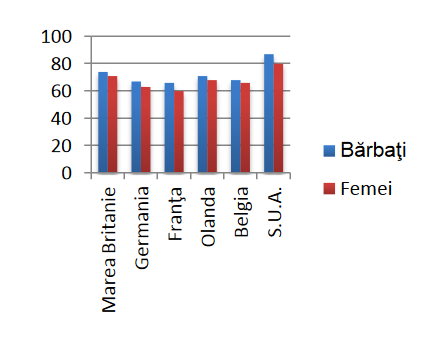
\includegraphics[scale=0.62]{fig1.png}
    \caption{Procente din popula\c{t}ie care aleg jocurile video.\footnotemark[1]}
  \end{subfigure}
  \begin{subfigure}{0.45\linewidth}
    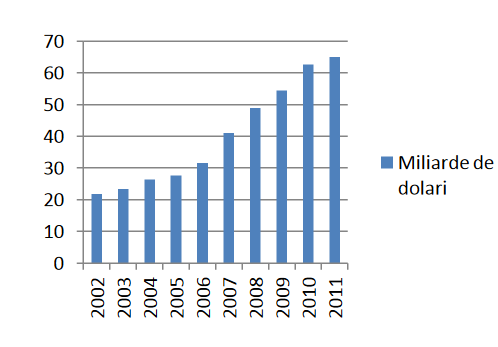
\includegraphics[scale=0.62]{fig2.png}
    \caption{C\^{a}\c{s}tigurile anuale ale industriei jocurilor video.}
  \end{subfigure}
\end{figure}


	De\c{s}i fiecare platform\u{a} pentru dezvoltarea jocurilor video are un rol important \c{s}i bine definit, aten\c{t}ia ne este atras\u{a} de dispozitivile mobile, \^{i}n special smarphone-uri \c{s}i tablete, a c\u{a}ror ramur\u{a} a cunoscut de-a lungul ultimilor ani o expansine extraordinar\u{a}.


	De la 17 ani de la lansarea primului smartphone modern de c\u{a}tre compania Nokia (modelul Nokia Communicator\footnotemark[2]) \c{s}i p\^{a}n\u{a} \^{i}n zilele noastre (a.c. 2013) num\u{a}rul de dispozitive mobile inteligente a dep\u{a}\c{s}it pragul de un miliard la nivel mondial, cre\c{s}tere care a adus odat\u{a} cu ea \c{s}i explozia pie\c{t}ei jocurilor video dedicate acestor dispozitive mobile.

	Pe l\^{a}ng\u{a} num\u{a}rul mare de dispozitive \c{s}i diversitatea categoriilor de jocuri disponibile, aceast\u{a} explozie se datoreaz\u{a} \c{s}i avantajelor pe care aceast\u{a} industrie le are asupra ``surorilor'' sale (industria jocurilor pentru calculatoare personale sau pentru console), at\^{a}t din punct de vedere al utilizatorului final, c\^{a}t \c{s}i din punct de vedere al dezvoltatorilor de jocuri.




\footnotetext[1]{ Sondaj online realizat de \textit{Today's Gamers} pe un e\c{s}antion de 13000 de persoane din \c{t}\u{a}rile men\c{t}ionate}
\footnotetext[2]{ Source: \url{https://en.wikipedia.org/wiki/Nokia_Communicator}}

\newpage
Printre aceste avantaje se numar\u{a}:

\begin{itemize}
	\item dimensiunea redus\u{a} a dispozitivelor care permite utilizatorilor s\u{a} se bucure de aplica\c{t}ii \^{i}n orice loc s-ar afla;
	\item modul de interac\c{t}ionare foarte intuitiv \c{s}i natural dintre dispozitiv \c{s}i utilizator prin intermediul ecranelor tactile sau accelerometrului;
	\item existen\c{t}a a\c{s}a numitelor market-uri care faciliteaz\u{a}din punct de vedere al utilizatorului achizi\c{t}ionarea jocurilor \c{s}i din punct de vedere al dezvoltatorului publicarea acestora;
	\item num\u{a}rul mare de unelte de dezvoltare pentru acest tip de aplic\c{t}ii mobile;
	\item pre\c{t}ul accesibil al aplica\c{t}iilor.
\end{itemize}


Astfel, nu este de mirare ca un studiu realizat recent de compania \textit{Flurry Analytics}\footnotemark[3] relev\u{a} faptul  c\u{a} jocurile sunt aplica\c{t}iile cele mai folosite de c\u{a}tre de\c{t}inatorii de dispozitive mobile inteligente.

\begin{figure}[h!]
 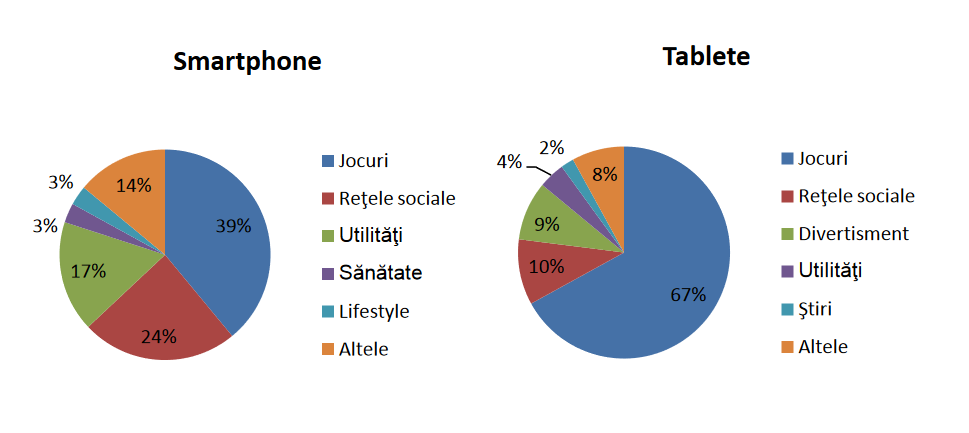
\includegraphics[scale=0.6]{fig3.png}
 \caption{Cele mai folosite aplica\c{t}ii pe dispozitivele mobile inteligente}
\end{figure}
 
\footnotetext[3]{ Source: \url{http://www.flurry.com/flurry-analytics.html}}
\end{document}